A programmable computer is a gadget without precedent.
It can be appreciated in many ways: %
through the constant stream of new flashy applications,
as an engineering marvel with continuous increase in performance and capacity,
or in the independent scientific discipline that forms its core~\cite{dijkstra1979a,hoare2006}.
For this dissertation, we focus on the intellectual challenge of \emph{programming} these gadgets.
\begin{quotation}
\noindent This challenge seems unique in the combination of the possibility for unmastered complexity -- programs are among the most
complex things ever conceived -- and the ultimate, but misleading, simplicity of a world of zeros and ones alone~\cite{dijkstra1979a}.
\end{quotation}

{Programming languages} provide us an interface that enable crafting programs.
The languages are an abstraction that relieve us from working directly with zeros and ones.
We write programs that are intended to be intelligible to humans.
Then, those programs are \enquote{translated} (compiled) into zeros and ones for processing by computers.
However, this abstraction does nothing to reduce the intellectual challenge involved in programming~\cite{dijkstra1979b}.
If we write a faulty program, we are at the mercy of our faulty creation (to be continued in~\autoref{verification}).

There is one feature about programs that has always fascinated me immensely.
It is that there are {multiple different ways} to write a program to compute the {same result}.
Essentially, we fix the inputs and expected output, but are free to change what happens in-between.
A scientifically inclined reader will recognize this concept as multiple algorithms computing the same function.
A software engineer will recognize it in the art of refactoring.
To demonstrate the idea, consider the two programs in~\autoref{lst:intro}.
The variable \pr|bit| is either \(0\) or \(1\).
It is clear the programs look different.
Yet, for all values of \pr|X| and \pr|Y|, I claim they compute the same result, stored in \pr|Z|.

\begin{center}
\captionsetup{type=lstlisting}
\begin{minipage}{.3\textwidth}
\lstinputlisting[nolol,label={lst:p1},frame=none,numbers=none,aboveskip=0pt,belowskip=0pt]{equiv1.imp}
\end{minipage}%
\hspace{3em}%
\begin{minipage}{.4\textwidth}
\captionsetup{type=lstlisting}
\lstinputlisting[nolol,label={lst:p2},frame=none,numbers=none,aboveskip=0pt,belowskip=0pt]{equiv2.imp}
\end{minipage}
\captionof{lstlisting}[Equivalent programs]{Equivalent programs.}
\label{lst:intro}
\end{center}

It is natural to ask, \emph{which program is better?}
The one on left reads more intuitively, making it easier to understand to a human.
Clarity is a useful criterion if the program is intended for frequent inspection.
The program on right has the advantage that it eliminates the conditional branching and evaluates in {constant time}.
These features are desirable, \eg for program security.
Choosing the preferable program form thus depends on semantics -- what do we mean by \emph{better}?

The purpose of the example is to help recognize that we can study programs as mathematical objects;
comparing their behaviors and quality attributes.
We should also confirm that the programs {actually} compute the same result instead of trusting an informal claim!
Thus, we need more than just abilities to \emph{write} programs.
Studying and reasoning about their \emph{behaviors} is an independent scientific challenge.

\subsection{Dissertation themes and topics}
\label{subsec:dissertation-themes}

Once we embrace the natural ambiguity of programs, we arrive to program analysis and formal methods.
These two are foundational topics of this dissertation.

Program analysis provides us the motivations to inspect programs and verify whether they satisfy some desirable criterion.
We call such criterion a \emph{property}.
A property is \emph{functional} if it relates to computation of the expected output.
Otherwise, a property is \emph{non-functional}.
Non-functional properties include quality attributes like security and resource consumption.
Broadly, the dissertation aims to analyze program properties through various \emph{syntactical} techniques.
In other words, we analyze how programs will behave when they are executed, based on the way programs are written and without executing them.
Formal methods complements the setting by adding the mathematical tools needed to obtain rigorous guarantees.
With formal methods it is possible to provide \emph{proofs} about the conclusions of program analysis.
This way, we can swap informal claims to maximally strong assertions.

To make the dissertation exploration more adventurous, and worthy of a multiyear doctoral study, we add
to the mix \emph{implicit computational complexity} (ICC).
Within the dissertation scope, the role of ICC is to provide a \enquote{toolbox} for constructing program analyses.
Briefly, ICC finds ways to characterize program properties (resource consumption) by introducing \emph{restrictions} at the level of programming languages.
It restricts what programs can be written in exchange for behavioral guarantees.
There are multiple compelling motivations for the ICC way of reasoning.
It drives better understanding and yields natural definitions and proofs of central results~\cite{kristiansen2017}.
It provides complementary and orthogonal techniques of program analysis, and delivers different kinds of results than alternatives.
Importantly, ICC enables reasoning about properties \emph{before} any program exists.
By this temporal shift, ICC empowers us to think about properties as part of programming language \emph{design}.
This removes the need for \emph{aposteriori} analysis of programs.

Combining the three topics gives us the full settings.
The dissertations is about \emph{analyzing} programs, ideally with \emph{formal guarantees}, and starting with a \emph{programming language}-based techniques that can provide guarantees by design.

\subsection{Addressed Problem}
\label{subsec:problem}

When we restrict a language, we will not be able to write every program -- \ie we sacrifice Turing-completeness.
This leads to the question, \emph{what can we do with such a language?}\footnote{
See \url{https://stackoverflow.com/questions/315340} for an inspirational warm-up.}
Every manuscript of this dissertation is an instance responding to this broader question.

The existing works in implicit computational complexity focus primarily on \emph{defining} theoretical systems that ensure desirable runtime properties;
typically, in terms of computational resource usage (\cf~\autoref{tab:icc-results}).
What separates this dissertation from those works is that it never defines such systems;
rather, it centers on \emph{applications}.
In this view, we take the existing ICC systems as a baseline---a kind of metaphorical \enquote{toolbox}---and assess their utility.
Each dissertation manuscripts approaches this task by combining implicit computational complexity with some other application domain.
The task of expanding ICC outside its traditional (theoretical) realm is difficult for at least three reasons.

\begin{enumerate}

\item Taking any pure theory and applying it reveals the shortcomings of the theory;
      and those issues must then be resolved.

\item Broad insight is required to first identify suitable application domains and to convert theories to applications.
Evidence supporting this statement can be found, \eg in automata theory\footnote{
The classic formulation of Parikh's Theorem concerns language expressiveness.
However, its usefulness in applications was enabled {only decades later}, by the development of efficient algorithms.
Parikh's Theorem has since then been exploited in a range of applications, including SMT solvers, verification of cryptographic protocols and concurrent programs, and query evaluation over graph databases, to name a few~\cite[pg. 2]{hague2024}}.

\item Presenting the applications requires communicating the findings to (new) audiences, who may be motivated differently to assess the {usefulness} of those findings.
\end{enumerate}

In other words, publishing findings involves a degree of technical evangelism.
Promoting implicit computational complexity to audiences who may have not encountered it previously, or at least not in the presented way, and getting them excited about its \emph{application} potential.
After many decades of theoretical development, the quest for applications is critical to move implicit computational complexity forward~\cite[p.~7]{moyen2017}.
Through the effort, we gain insight of the technical power, limitations, and benefits of ICC systems as compared to alternative techniques;
as the manuscripts in this dissertation will demonstrate.

\begin{figure}[t]
\begin{mdframed}
\paragraph*{Main hypothesis.}
Implicit computational complexity offers applied utilities when lifted outside the theoretical domain.
\end{mdframed}
\caption[Main hypothesis summarized]{Main hypothesis.}
\label{fig:hypothesis}
\end{figure}

\subsection{Dissertation Goals}\label{subsec:specific-aims}

This dissertation has four goals.

\begin{enumerate}
\item Extend \emph{applied} capabilities of ICC in automatic program analysis and verification.
\item Take ICC-bases analyses a few steps closer to becoming a standard in real world development workflows.
\item Initiate discourse on relevance of applications within the ICC community.
\item Expose ICC-based analyses to broader research communities.
\end{enumerate}

The first is to demonstrate that implicit computational complexity is useful in \emph{automated} complexity analysis.
Despite many compelling features, implicit computational complexity has remained primarily as a theoretical novelty.
The purpose of the goal is to address this limitation.
All too often practitioners regard theory as irrelevant, and theoreticians think of practice as trivial~\cite[pg. xxxv]{bishop2003}\footnote{
For example, for papers with implementations, the inability to demonstrate a practically functional artifact is a not a disqualifying factor for a top-conference publication,
\cf\eg~\url{https://artifact-eval.org/motivation.html}.}.
The previous statement is loaded, but it needs to be states as a founding motivation of the dissertation.
In our view~\cite[p. 75]{moyen2017}, theory and applications are symbiotic.
Investigations of both are needed for scientific advancement.
This goal corresponds to a series of manuscripts that extend the flow calculus of mwp-bounds (\autoref{flow-calculus}).

The last two goals are social.
% TODO: finish this thought

%A guiding intuition behind these goals is that, {if applied}, implicit computational complexity could provide new practical program analyses.
%These include uses in formal verification and in specifying and ensuring \uline{many} non-functional properties.

% \subsection{Significance}\label{subsec:significance}
% This research proposal intersects computer science theory and application, with the intent of using those theoretical approaches to solve existing challenges in automatic program analysis.
% In 2017, Jean-Yves Moyen---a notable researcher in the ICC community, whose career spans 3 decades of advancements---remarked enthusiastically, that after twenty years and many results, ICC was ready to move into real-world and to concrete applications~\cite[p.~7]{moyen2017}.
% And although a few early results exist, as noted earlier in this section, progress in this direction is still at early stages.
% With similar aspirations, this proposal hopes to move further in that direction.
% It is conceivable that certified complexity would be of significant interest to multiple research communities.
% The next section will detail the specifics of the methodology, that consists of multiple projects.
% Assuming the successful completion of each project, they would show that certifiably correct complexity analysis is achievable, and that ICC techniques can be used to obtain efficient and practical complexity analysis.
% These results would extend current capabilities in automatic complexity analysis, and move those techniques closer to becoming a standard in real-world software verification.

\subsection{Overview of Manuscripts and Research Questions}
\label{subsec:conn-papers}

\begin{figure}[p]
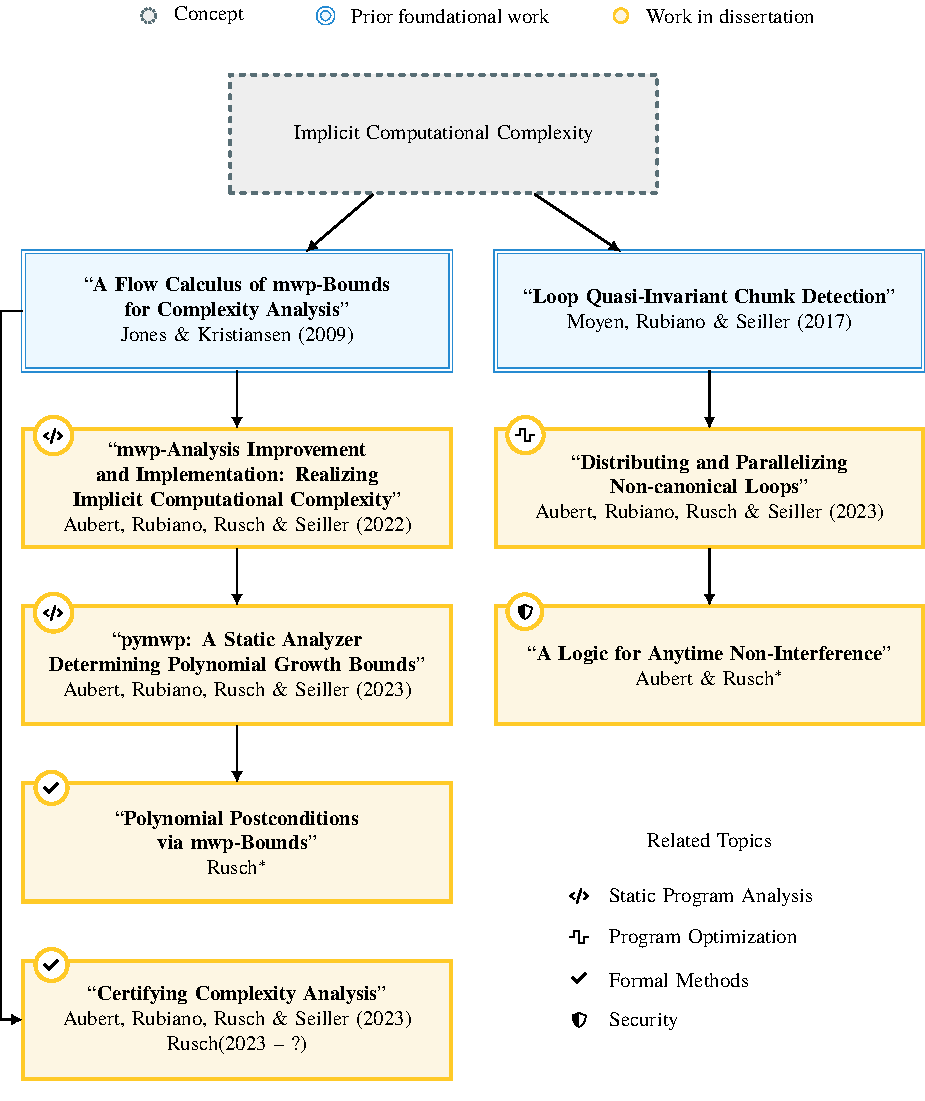
\includegraphics[width=\linewidth,keepaspectratio]{fig_conn_papers}\vspace{1em}
\caption[Dissertation manuscripts and their associations]
{Dissertation manuscripts and their associations.}
\label{fig:conn_papers}
\end{figure}

All dissertation manuscripts are inspired by theoretical works in implicit computational complexity.
Based on the foundation, the manuscripts are organized into two \enquote{paths}, as shown in~\autoref{fig:conn_papers}.
The paths align with the dissertation goals (\autoref{subsec:specific-aims}) as follows.

\begin{description}
\item[Automatic resource analysis with the flow calculus of mwp-bounds.]
The first track extends the flow calculus of mwp-bounds of~\textcite{jones2009}.
The technique is introduced detail in~\autoref{flow-calculus}.
The flow calculus is a syntactical analysis for reasoning about variable value growth during computation.
The manuscripts apply and demonstrate the utility of the calculus, first though static program analysis, then extending it to formal methods.
Thus, the manuscripts supports two of the three dissertation goals.
One of the manuscripts is in the appendix due to the university policies, but the placement should not distract from its significance;
several other manuscripts follow from it.

\begin{description}
\item[RQ1] Can we develop an \emph{automatic} program analysis based on the theory?
\item[RQ2] Given its paper proofs, is the theory correct? Can we prove formally the soundness of the flow calculus?
\item[RQ3] Assuming the theory can be automated, what are the use cases of the analysis?
\end{description}

\item[Analyzing extended program properties via quasi invariants.]
The second track is inspired by \enquote{Loop Quasi-Invariant Chunk Detection}~\cite{moyen20172}.
The idea is to identify blocks of code in loops that become invariant after some finite number of loop iterations.
These quasi-invariant blocks can then be lifted from the loop to ideally improve the loop's complexity profile.
The manuscripts in this track support the second dissertation goal,
as they use the mathematical framework of LQICM to track other program properties.
In particular, they show how to adjust the mathematics to obtain a program optimization to increase parallelism and detect the security property of non-interference.

\begin{description}
\item[RQ4] How to develop a program transformation to increase parallelization potential?
\item[RQ5] How to use it to analyze security properties, specifically non-interference?
\end{description}

%The second goal is to show that the analytical techniques developed around implicit computational complexity extend to analyzing \emph{other} semantic program properties.
%This goal shows that ICC-based analyses are flexible enough to extend beyond their original design.
%Although the goal is phrases in terms of \emph{properties}, the emphasis is actually on the \emph{techniques} and understanding how they adjust to providing various guarantees.
%The boarded implications suggests that viewing ICC as a niche sub-field of complexity theory does not adequately recognize its true analytical power.
%The various ways in which ICC analyses can provide guarantees should be explored more broadly.
%The manuscripts in this dissertation demonstrate two use cases in program optimization and security analysis.
      
\end{description}

\paragraph*{Related topics.}
Each manuscript relates implicit computational complexity with some other research topic.
The topics include: static program analysis, security, program optimization, and formal methods.
Throughout the dissertation, each manuscript is decorated with a icon that denotes the primary related topic.

\paragraph*{On manuscript authorship.}
The manuscript authors are listed in alphabetical order.
The manuscripts in Chapters~\ref{published-manuscripts}--\ref{ch:unpublished-research} are \enquote{first author} works,
and manuscripts in~\autoref{app:additional-manuscripts} are \enquote{non-first author} works.
The contributions of the co-authors are detailed in~\autoref{app:sec:coauth}.

\paragraph*{On manuscript peer review.}
The entire Chapters~\ref{published-manuscripts},~\ref{ch:unpublished-research},~\ref{ch:summary}, and ~\ref{app:additional-manuscripts}
has been previously peer-reviewed.
The published works, in Chapters~\ref{published-manuscripts} and~\ref{app:additional-manuscripts}, were inspected by 7--10 reviewers before acceptance.
The unpublished works, in \autoref{ch:unpublished-research}, have been reviewed by 3--6 reviewers thus far.
However, the unpublished research requires a word of caution.
By implication, they all have some limitation that prevents them from being in the {published} manuscripts-chapter.
Preliminary versions of most unpublished works have been accepted and presented at respectable workshops.
\autoref{ch:summary} is a stand-alone extended abstract about the entire dissertation.
It has been peer-reviewed as a submission at a doctoral symposium.

\subsection{Important Tips for Interacting With This Document}
\label{subsec:tips}

This dissertation contains three versions of its contents.
The versions differ in length.
Read the version that best matches your needs and time constraints.

\begin{mdframed}[backgroundcolor=priorbase,linecolor=cc]
\begin{enumerate}[wide, labelwidth=!, labelindent=0pt]
\item The \hyperref[abs]{abstract}:covers the highlights only.
\item Chapters~\ref{introduction}--\ref{ch:discussion} and \ref{app:additional-manuscripts}: the full length presentation.
\item \autoref{ch:summary}: an extended, standalone abstract of the full presentation.
\end{enumerate}
\end{mdframed}

\subsubsection{Software Artifacts and Data Availability}

Each published and publication-ready manuscript---including the dissertation itself---comes with a software artifact.
In other words, each manuscript consists of more than {just the text pages} of this dissertation.
All software developed as part of this dissertation is publicly available.
How to locate the associated software is explained in~\autoref{app:sec:artifacts}.
The software is archived for long-term retention according to the policies of the Association for Computing Machinery~\cite{acm_badging}.
The software is achieved even if the publication venue did not have an official artifact evaluation round.

\subsubsection{Notational Conventions}

\paragraph*{Code blocks and line numbers.}
Inlined syntactic constructs (variables, expressions, commands, \etc) are typeset in \texttt{teletype}.
Larger code blocks are displayed in dedicated listings.
The listings will display, in bottom right corner, the associated programming language (or context) according to~\autoref{tab:pls}.
In the table, \emph{Version} is the release version assumed in the dissertation listings.
Pseudo-languages have no version.
Plain text listings, that describe command outputs, are labelled \enquote{output}.
The Rocq Prover (formerly Coq) is actively undergoing a name change.
Whenever possible we refer to the new name.

\begin{table}[h]
\begin{center}
\begin{tabular}{@{}lllc@{}}
\toprule
\multicolumn{2}{@{}l}{\textbf{Language}} & \textbf{Description} & \textbf{Version} \\
\midrule
\langclr{cc}        & C     & C language & C99 \\
\langclr{ccstar}    & C*    & imperative C-like pseudo-language & -- \\
\langclr{cces}      & CES   & cost equation system &  -- \\
\langclr{ccmd}      & cmd   & executable shell (terminal) command & --  \\
\langclr{cdafny}    & Dafny & Dafny language & 4.10.0 \\
\langclr{cimp}      & Imp   & imperative language of mwp-calculus & -- \\
\langclr{cjava}     & Java  & Java language & SE 24 \\
\langclr{compcode}  & OMP   & C code that includes OpenMP directives & 6.0 \\
\langclr{crocq}     & Rocq  & Roqc interactive theorem prover & 9.0.0 \\
\langclr{cmathc}    & SSR   & the SSReflect proof language & 2.3.0 \\
\langclr{cwhile}    & While & simple imperative while language & -- \\
\bottomrule
\end{tabular}\end{center}
\caption[The programming languages of code listings]{The programming languages used in code listings.}
\label{tab:pls}
\end{table}

References to specific line of source code, or an algorithm, begin with L, for \underline{l}ine.
The L is followed by a number (or a numeric range) that specifies the rows of interest.
For example, L3 means \enquote{line number 3}, and L10--12 means \enquote{lines 10 through 12}.

\paragraph*{Distinguishing variable states.}
We will often want to refer to the same variable in different states of computation.
In the style of the Z specification language\index{Z specification language}~\cite{spivey1992},
we use notation that identifies the \emph{new (post) states}.
A plain variable refers to a state where the variable holds its \emph{initial} value.
A variable with a postfix decoration \pr|'| refers to a state where the variable holds its \emph{final} value.
For example, \pr|X| refers to the initial value, and \pr|X'| refers to the final value.

\subsubsection{Term and Notational Indices}

This dissertation includes three indices.
The Term Index (\autoref{sec:app:index}) lists technical terms and their most relevant uses.
Acronyms are generally defined at first-use.
After that, it is always possible to locate the long form in the index of acronyms (\autoref{glo:acr}).
A similar lookup reference is available for symbolic notations (\autoref{glo:symb}).

\subsubsection{Dynamic Bibliographic Entries}

Some bibliography entries refer to resources that are not traditional scientific papers --
like software, web pages, lecture notes, and technical reports.
To improve long-term availability of such dynamic entries, a backup is deposited in well-established online archives.

\begin{description}
\item[Written documents.]
Web pages and PDF files are archived at the Internet Archive.
To recover a document, substitute \pr|<URL>| by the document's URL.
\begin{center}\pr|https://web.archive.org/web/<URL>|\end{center}

\item[Software repositories.]
Version-controlled third party software repositories are archived by \href{https://softwareheritage.org/}{Software Heritage}.
For a repository at \pr|<URL>|, the recovery address is:%
\begin{center}\pr|https://archive.softwareheritage.org/browse/origin/directory/|\mbox{\pr|?origin_url=<URL>|}\end{center}
\end{description}

Documents that were not readily available online even at the time of writing this dissertation, are archived in the dissertation companion artifact (\autoref{tab:pub-artifacts}).

\paragraph*{Recovering archived documents.}
For example, the following \href{https://types22.inria.fr/files/2022/06/TYPES_2022_paper_14.pdf}{URL} is fragile and may disappear in the future.

\begin{center}
\begin{minipage}{\textwidth}
%! suppress = EscapeUnderscore
\begin{cmdlisting}*[nolol]
https://types22.inria.fr/files/2022/06/TYPES_2022_paper_14.pdf
\end{cmdlisting}
\end{minipage}
\end{center}

If a request of the original document fails, the \href{https://web.archive.org/web/https://types22.inria.fr/files/2022/06/TYPES_2022_paper_14.pdf}
{corresponding Internet Archive address} produces the same document.

\begin{center}
\begin{minipage}{\textwidth}
%! suppress = EscapeUnderscore
\begin{cmdlisting}*[nolol]
https://web.archive.org/web/https://types22.inria.fr/files/2022/06/TYPES_2022_paper_14.pdf
\end{cmdlisting}
\end{minipage}
\end{center}